\documentclass[tikz,border=10pt]{standalone}
\usepackage{amsmath}
\usepackage{tikz}
\usetikzlibrary{matrix, positioning, arrows.meta, decorations.pathreplacing, calc, fit}

\begin{document}
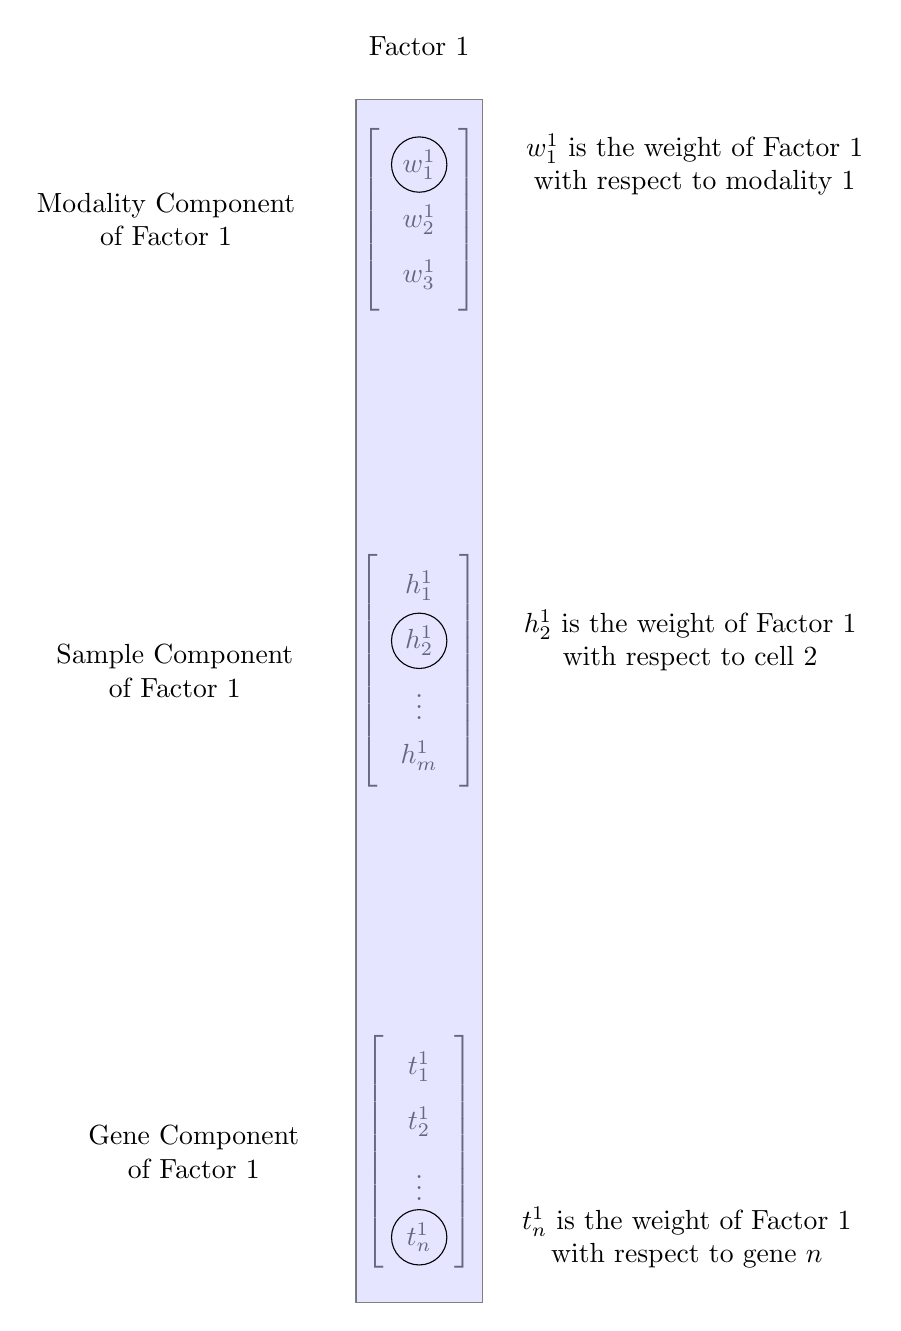
\begin{tikzpicture}[>=Stealth]

  % Define matrix styles
  \tikzset{
    vector style/.style={
      matrix of math nodes,
      nodes={minimum width=5mm, minimum height=7mm, anchor=center},
      left delimiter=[,
      right delimiter=],
    }
  }

  % Experimental factors vector
  \matrix (v1) [vector style] at (0,0) {
    |(w11)| w_1^1 \\
    w_2^1 \\    
    w_3^1 \\
  };
  \node[align=center, left=10mm of v1] {Modality Component \\of Factor 1};
  \node[above=9mm of w11] {Factor 1};

  % Sample factors vector
  \matrix (p1) [vector style, below=3cm of v1] {
    h_1^1 \\
    |(h12)| h_2^1 \\
    \vdots \\
    h_m^1 \\
  };
  \node[align=center, left=10mm of p1] {Sample Component \\of Factor 1};

  % Genomic factors vector
  \matrix (g1) [vector style, below=3cm of p1] {
    t_1^1 \\
    t_2^1 \\
    \vdots \\
    |(t1n)| t_n^1 \\
  };
  \node[align=center, left=10mm of g1] {Gene Component \\of Factor 1};
  \node[draw, fill=blue!20, opacity=0.5, fit=(v1)(g1), inner sep=10pt] (factor_one) {};



% Draw circle around w_1^1
\draw (w11) circle [radius=10pt];
\draw (h12) circle [radius=10pt];
\draw (t1n) circle [radius=10pt];

  % Labels for Factor 1 entries
  \node[right=9mm of w11, align=center] {$w_1^1$ is the weight of Factor 1\\ with respect to modality $1$};
  \node[right=9mm of h12, align=center] {$h_2^1$ is the weight of Factor 1\\ with respect to cell $2$};
  \node[right=9mm of t1n, align=center] {$t_n^1$ is the weight of Factor 1\\ with respect to gene $n$};
  
\end{tikzpicture}
\end{document}
